\section{Robot Gripper}


\begin{figure}[H]
    \centering
    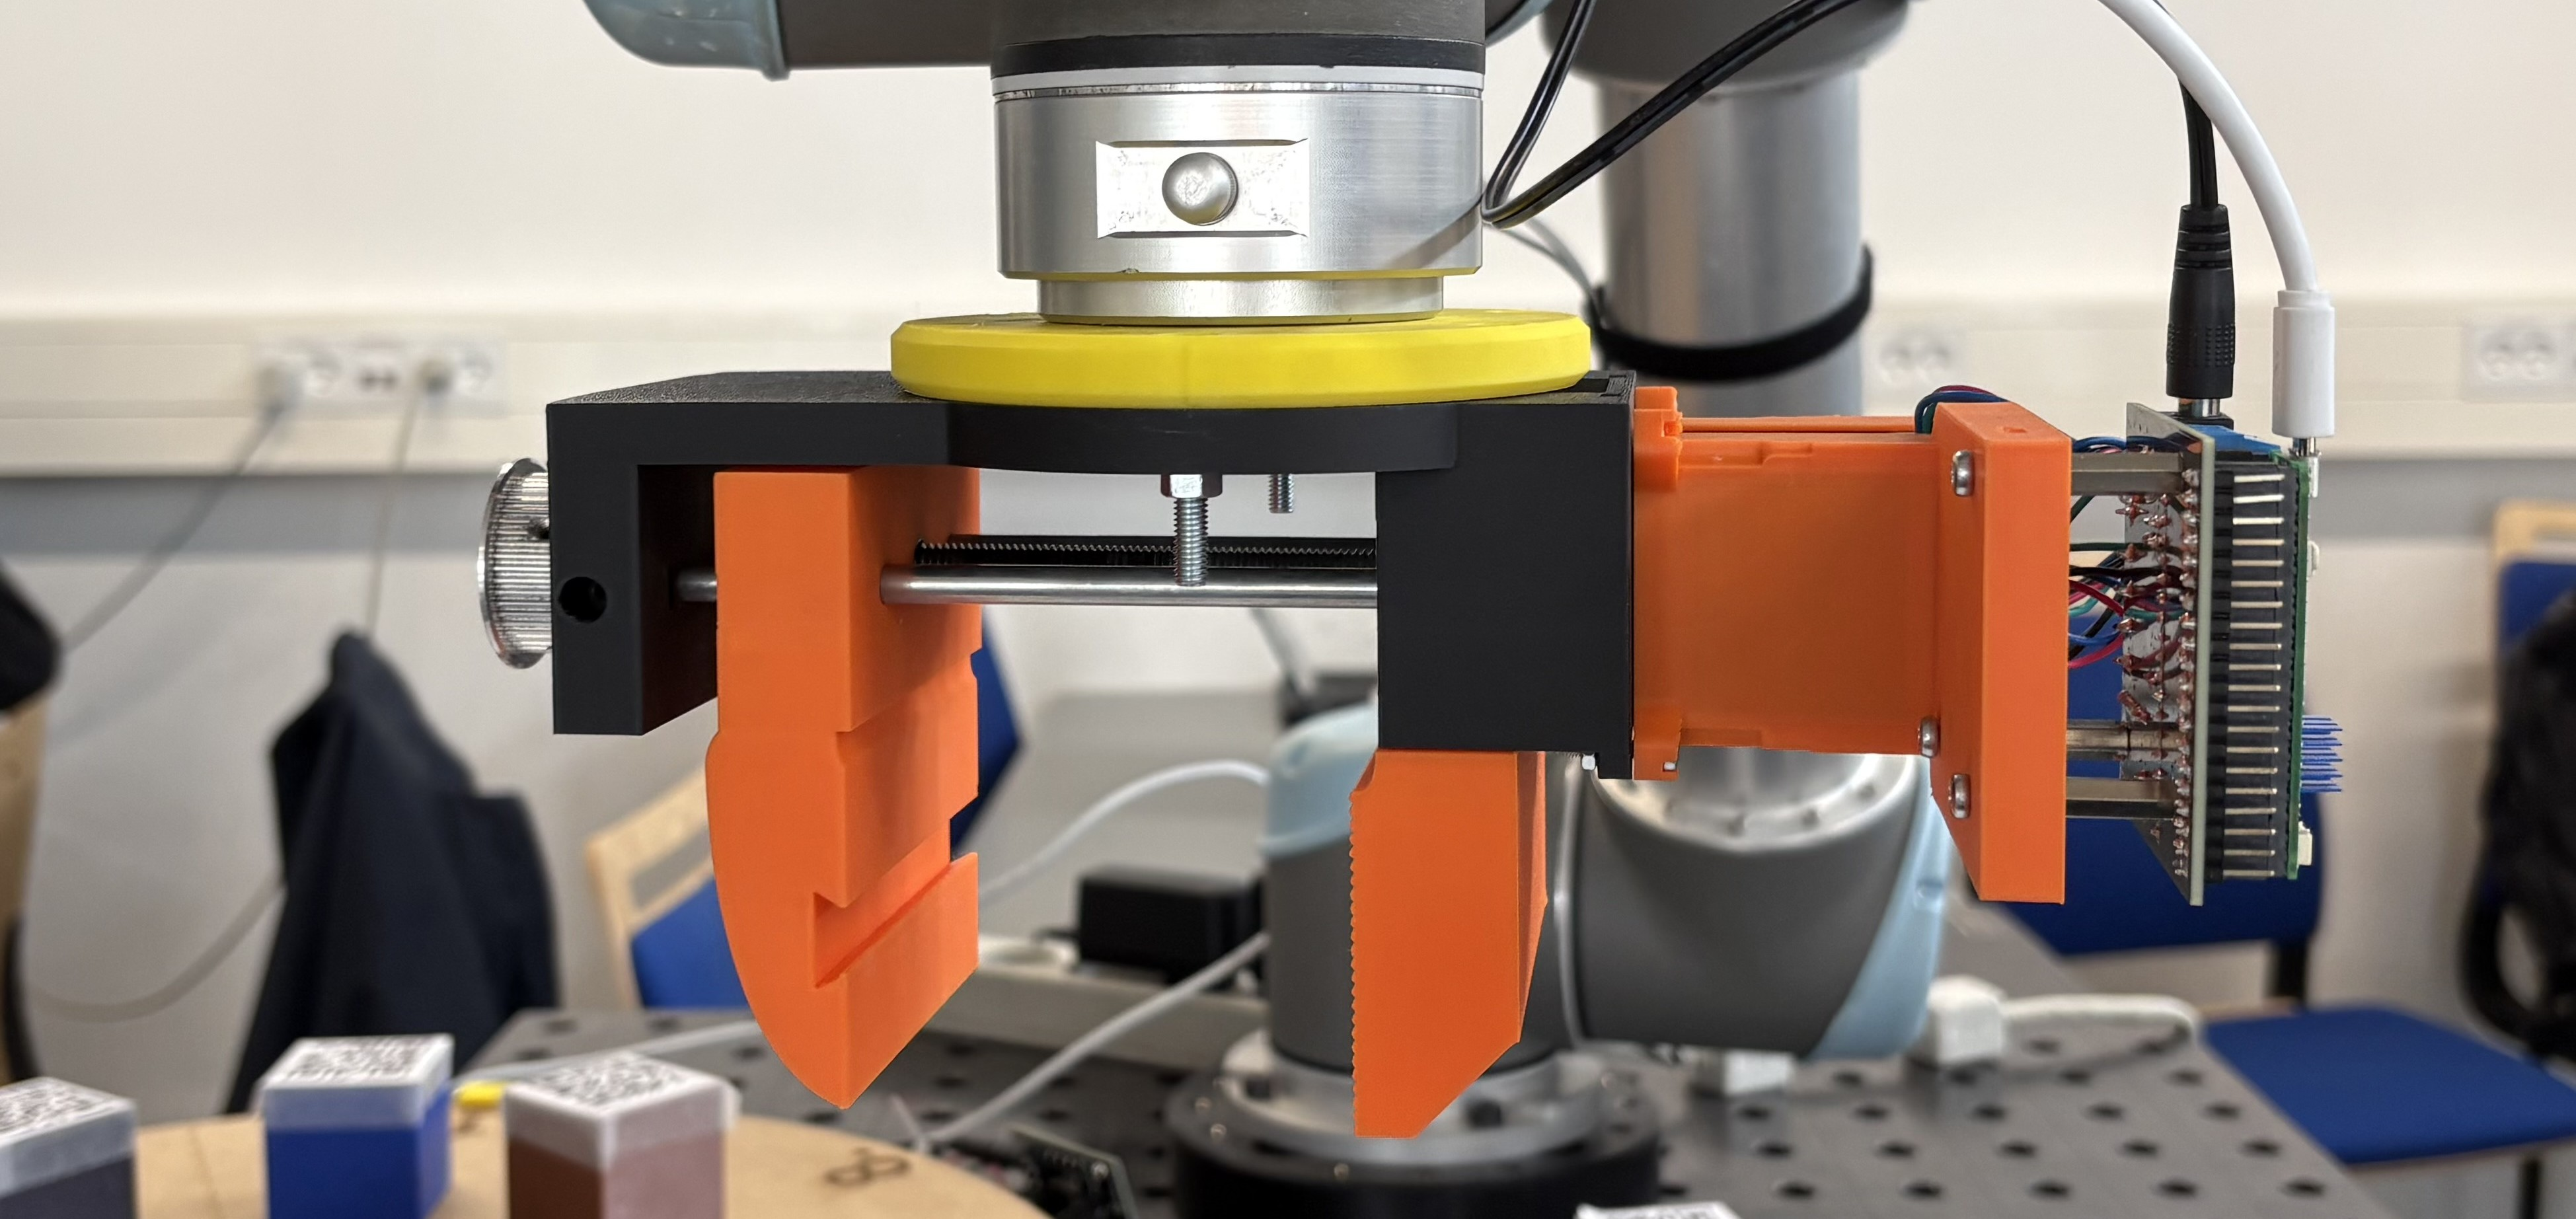
\includegraphics[width=0.75\textwidth]{figures/Gripper.jpeg}
    \caption{Final robot gripper design}
    \label{fig:gripper-design}
\end{figure}


The robot gripper is responsible for physically picking up, holding, and releasing objects. The gripper was designed to handle objects with different dimensions while keeping the contact surfaces parallel throughout the gripping motion. In the initial design phase, a linkage based parallel gripper was considered, since this type of mechanism can keep both gripper fingers parallel while opening and closing. This would have made it possible to grip objects of different sizes with a consistent contact geometry.

The final construction instead uses a simpler linear screw mechanism, where one side of the gripper moves linearly while the opposite side remains fixed. The screw is driven by a stepper motor through a spring coupling. The spring coupling was not ideal for the stall detection strategy, because it can absorb part of the mechanical load before the motor detects the stall. It was still used because it was the available coupling for the construction. The effect of this on the stall detection is discussed later in this section.

A stepper motor was selected because its discrete steps provide a useful reference for estimating the gripper movement. Combined with stall detection at the end stop, this allows the software to reset the gripper to a known mechanical position and then use step counts for subsequent movements.

A custom PCB was designed for the gripper to integrate the microcontroller, stepper driver, and current measurement circuit. The PCB layout and schematic can be seen in Appendix~\ref{app:gripper-pcb}. The current measurement circuit uses a shunt resistor in series with the stepper driver supply, which is also the supply path that provides power to the motor. This makes it possible to measure the small voltage drop across the resistor and use it to estimate the motor current. The voltage is amplified by a current sense amplifier IC so the microcontroller can read it through its internal ADC.



\subsection{Software}
\label{sec:gripper-software} %Reference used in storage
\begin{figure}[H]
    \centering
    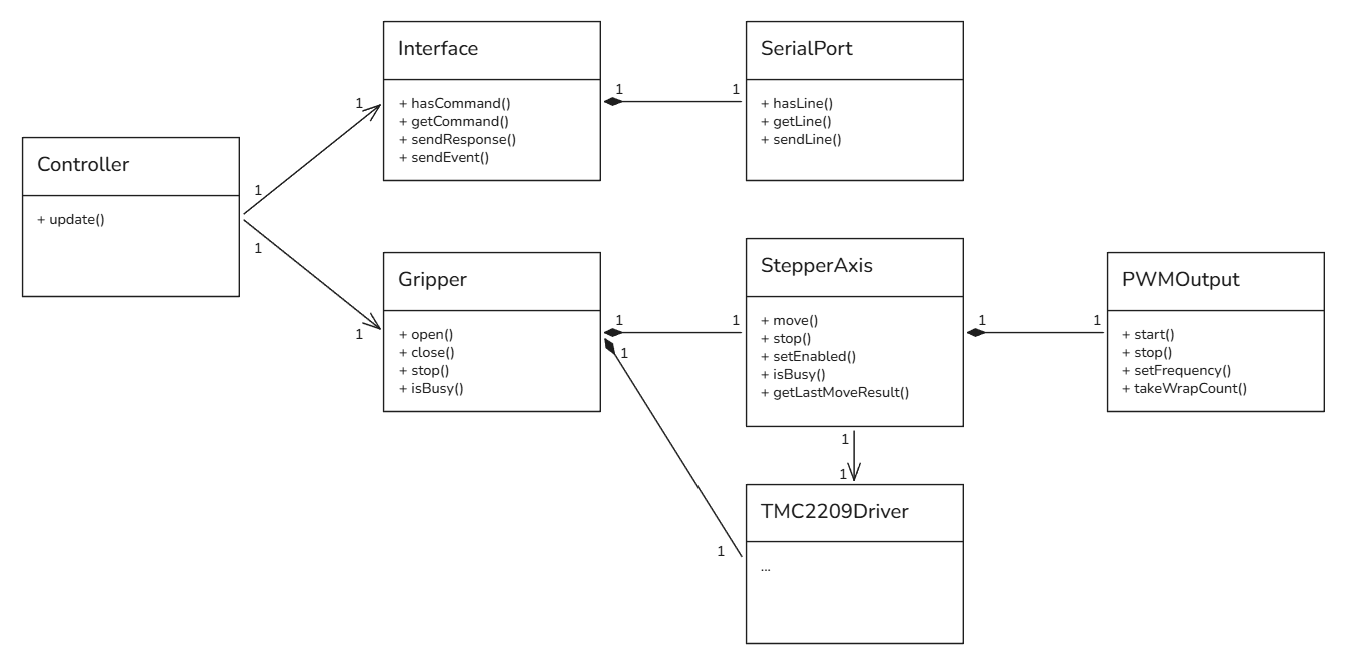
\includegraphics[width=1\textwidth]{figures/diagrams/GripperClass.png}
    \caption{Gripper class diagram}
    \label{fig:gripper-class}
\end{figure}

The software for the gripper was implemented on the microcontroller as a small layered control system. The purpose of this structure was to keep the external command interface separated from the motor control and low level hardware access. This makes the system easier to test and makes it possible to change individual parts without rewriting the rest of the software.

The class structure is shown in \cref{fig:gripper-class}. The \texttt{Controller} is the top level of the microcontroller program. It checks for new commands, calls the relevant function in the gripper logic, and sends responses and events back to the PC. The \texttt{Interface} class parses incoming command lines and formats outgoing responses, while \texttt{SerialPort} handles the line based serial communication.

The \texttt{Gripper} class contains the state machine for the mechanism. It exposes high level functions such as \texttt{open()}, \texttt{close()}, \texttt{stop()}, and \texttt{isBusy()}, and translates these actions into one or more motor movements. For example, an open command can include a reset movement against the rear stop followed by a short forward movement. This makes the gripper return to a known mechanical position instead of relying only on an assumed step count.

The actual stepper movement is handled by \texttt{StepperAxis}. This class controls direction, tracks the remaining steps, updates the speed profile, and decides whether a movement has ended by completing its step count, being stopped, or detecting a stall. Below this layer, \texttt{PWMOutput} generates the step pulses for the motor driver, and \texttt{TMC2209Driver} configures and reads feedback from the TMC2209 driver over UART. This separation means that the high level gripper logic does not depend directly on how PWM pulses or driver registers are implemented.

\begin{figure}[H]
    \centering
    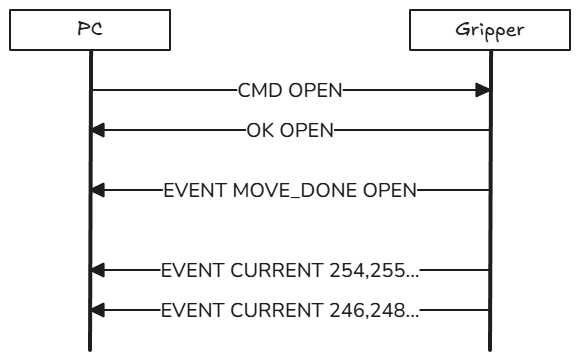
\includegraphics[width=0.6\textwidth]{figures/diagrams/ComsSequance.png}
    \caption{Communication sequence diagram}
    \label{fig:gripper-communication-sequence}
\end{figure}

The communication between the PC and the microcontroller is based on text strings sent over serial. The PC sends command lines starting with \texttt{CMD}, such as \texttt{CMD OPEN}. The gripper first replies with an acknowledgement, for example \texttt{OK OPEN}, to show that the command was accepted and started. When the movement has finished, it sends a separate event such as \texttt{EVENT MOVE\_DONE OPEN STALL}. In this event, \texttt{MOVE\_DONE} describes what event happened, \texttt{OPEN} shows which command or movement the event belongs to, and the final field explains why the movement ended, for example \texttt{STALL}, \texttt{STEPS\_FINISHED}, or \texttt{STOPPED}. This makes the interface usable in the complete system because the PC can wait for a movement event before starting the next robot action.

The same interface is also used for measurement data. The current sensor samples the motor current during operation and sends batches of samples as event messages. In the implemented version, the current was sampled every 20 ms and sent in batches of five samples. This gives the PC access to measurement data without requiring a separate request for every sample. The format is:

\begin{center}
\texttt{EVENT CURRENT <start\_ms> <sample\_period\_ms> <values...>}
\end{center}

\subsection{Stall detection}

Detecting a stall is a central part of the gripper software. The gripper is a linear mechanism, and it uses mechanical resistance as a signal. When the gripper closes around an object, the motor load rises because the fingers can no longer move freely. The same principle is used during reset, where the gripper moves against the rear stop to find a known reference position.

Two stall detection methods were implemented and compared. The first method used StallGuard from the TMC2209 motor driver\cite{tmc2209_datasheet}. In this mode, the microcontroller reads the driver over UART while the motor is moving. The software filters the StallGuard result and only accepts a stall after the signal has passed the configured threshold for several consecutive samples. This avoids stopping on a single noisy reading.

The second method used the measured motor current. The expected behaviour was that the current would increase when the gripper reached an object or endstop. However the measured current could contain short peaks that crossed the threshold in normal running and that could be mistaken for a stall. To reduce the effect of these peaks, the software averaged multiple current samples before comparing the result with the threshold. A stall was only accepted after the averaged current had exceeded the threshold for several repeated checks.

The stall detection depends on how directly the load is transferred from the gripper jaws to the motor. In this design, a spring coupling was used between the motor and the screw mechanism. When the gripper closes around an object, the spring coupling can extend as the gripping force increases, so part of the jaw movement is absorbed before the motor load rises enough for a stall to be detected. This makes the stall response slower and less distinct. The difference can be seen by comparing the spring coupled gripping measurement with the hardstop measurement in Appendix~\ref{app:stall-charts}, where \cref{fig:stall-chart-with-spring} shows the softer response during gripping and \cref{fig:stall-chart-hard-stop} shows the sharper response against the hard stop. Because of this, the spring coupling was not ideal for this type of stall detection, and a stiffer coupling would likely have made the gripper response easier to detect.

The final version uses the StallGuard method. The current-based method was useful for logging and for understanding the motor behaviour, but it was harder to tune as the stall condition. The threshold had to be high enough to avoid reacting to remaining short current peaks after averaging, but low enough to detect a stall before the stepper motor started overstepping. Finding a suitable balance between these requirements was difficult without introducing at least one of the drawbacks. This made the method less reliable, so it was not chosen for the final version.

\subsection{Evaluation}

The gripper was evaluated with repeated open and close sequences. Each test run consisted of a close movement, an open movement, a reset movement against the open end stop, and a short forward movement away from the stop. A run was counted as failed if any movement in the sequence did not finish with the expected result, such as failing to detect an expected stall or detecting a stall during a movement that should have completed freely.

Two sets of 50 runs were performed using StallGuard with different parameter settings. In total, this gave 100 tested sequences. All 100 StallGuard runs completed without a failed sequence. This showed that the driver based stall signal was repeatable enough for both gripping and reset detection.

The current based stall detection was tested with one set of 50 runs. In this test, one sequence failed because the gripper overstepped and the software did not detect the stall correctly. In six additional cases the stepper motor lost torque at stall, which caused overstepping, but the sequences still completed and were therefore not counted as failed runs. This can be seen in \cref{fig:stall-chart-with-overstepping} in Appendix~\ref{app:stall-current-overstepping}.

\begin{table}[H]
\centering
\small
\begin{tabular}{|p{0.23\textwidth}|p{0.12\textwidth}|p{0.12\textwidth}|p{0.35\textwidth}|}
\hline
Detection method & Test runs & Failed runs & Observations \\
\hline
StallGuard & 100 & 0 & No failed sequences \\
\hline
Current threshold & 50 & 1 & Six overstepping cases without fail \\
\hline
\end{tabular}
\caption{Gripper stall detection test results.}
\label{tab:gripper-stall-detection-results}
\end{table}

Based on these tests, StallGuard was selected as the final stall detection method. The current measurement signal was still useful as diagnostic data, but it was not reliable enough as the primary control signal. The StallGuard method gave a clearer stop condition and was easier to tune for repeated operation.
